\documentclass[../../informe/src/main.tex]{subfiles}

\begin{document}
	\section{Ejercicio 2}
	Se tiene la siguiente expresión en maxtérminos $f(d;c;b;a) = \prod_{}^{}(M_{0};M_{1};M_{5};M_{7};M_{8};M_{10};M_{14};M_{15})$ \par
	De aquí se desprende la siguiente tabla de verdad, de la cual se derivan las expresiones completas en función de las entradas.
	%tabla de verdad para las entradas.
	\begin{table}[H]
		\centering
 			\begin{tabular}{||c c c c c c c||} 
 				\hline
				d & c & b & a & - & f & $M_{i}$\\ [0.5ex] 
 				\hline\hline
 					0 & 0 & 0 & 0 & - & 0 & $M_{0}$ \\
 					0 & 0 & 0 & 1 & - & 0 & $M_{1}$ \\
 					0 & 0 & 1 & 0 & - & 1 & $M_{2}$ \\
 					0 & 0 & 1 & 1 & - & 1 & $M_{3}$ \\
 					0 & 1 & 0 & 0 & - & 1 & $M_{4}$ \\
 					0 & 1 & 0 & 1 & - & 0 & $M_{5}$ \\
 					0 & 1 & 1 & 0 & - & 1 & $M_{6}$ \\
 					0 & 1 & 1 & 1 & - & 0 & $M_{7}$ \\
 					0 & 0 & 0 & 0 & - & 0 & $M_{8}$ \\
 					0 & 0 & 0 & 1 & - & 1 & $M_{9}$ \\
 					0 & 0 & 1 & 0 & - & 0 & $M_{10}$ \\
 					0 & 0 & 1 & 1 & - & 1 & $M_{11}$ \\
 					0 & 1 & 0 & 0 & - & 1 & $M_{12}$ \\
 					0 & 1 & 0 & 1 & - & 1 & $M_{13}$ \\
 					0 & 1 & 1 & 0 & - & 0 & $M_{14}$ \\
 					0 & 1 & 1 & 1 & - & 0 & $M_{15}$ \\ [1ex] 
 				\hline
  	\end{tabular}
	\end{table} \par
	
	%expresion en términos de los bits de entrada
	Expandiendo la expresión, f =$ (d+c+b+a)\cdot (d+c+b+\overline{a})\cdot (d+\overline{c}+b+\overline{a})
	\cdot (d+\overline{c}+\overline{b}+\overline{a})\cdot (\overline{d}+c+b+a)\cdot
	 (\overline{d}+c+\overline{b}+a)\cdot (\overline{d}+\overline{c}+\overline{b}+a)\cdot
	 (\overline{d}+\overline{c}+\overline{b}+\overline{a})$
	 \par
	 \begin{enumerate}
	 %simplifación por álgebra booleana:
	 	\item Simplificamos mediante el uso del álgebrea booleana: \par
	 	
	 	%primera simplificación - Combining 14.b
	 		Agrupando a los maxtérminos anteriores de a dos y en orden, aplicando la propiedad 14.b del álgebra de Boole de la página del 				libro ''Fundamentals of Digital Logic with Verilog Design'' propuesto por la cátedra, la expresión queda simplificada a: \par
	 		f =$ (d+c+b)\cdot (d+\overline{c}+\overline{a})\cdot (\overline{d}+c+a)\cdot (\overline{d}+\overline{c}+\overline{b})$\par
			
			Esta resulta ser la mínima expresión de f. \par

			
	%simplifación por álgebra booleana:
		\item Simplificamos mediante el uso de mapas de Karnaugh: \par

 			\begin{table}[H] %Karnaugh general
				\centering
 				\begin{tabular}{||c c c c c||} 
 					\hline
					$b$,$a$|$d$, $c$ & 00 & 01 & 11 & 10\\ [0.5ex] 
 					\hline\hline
					00 & $M_{0}$ & $M_{4}$ & $M_{12}$ & $M_{8}$\\
					01 & $M_{1}$ & $M_{5}$ & $M_{13}$ & $M_{9}$\\
					11 & $M_{3}$ & $M_{7}$ & $M_{15}$ & $M_{11}$\\
					10 & $M_{2}$ & $M_{6}$ & $M_{14}$ & $M_{10}$\\[1ex] 
					\hline
				\end{tabular}
			\end{table}
			\begin{itemize}
				\item $f$
					\begin{figure}[H]	%Circuito
						\centering
						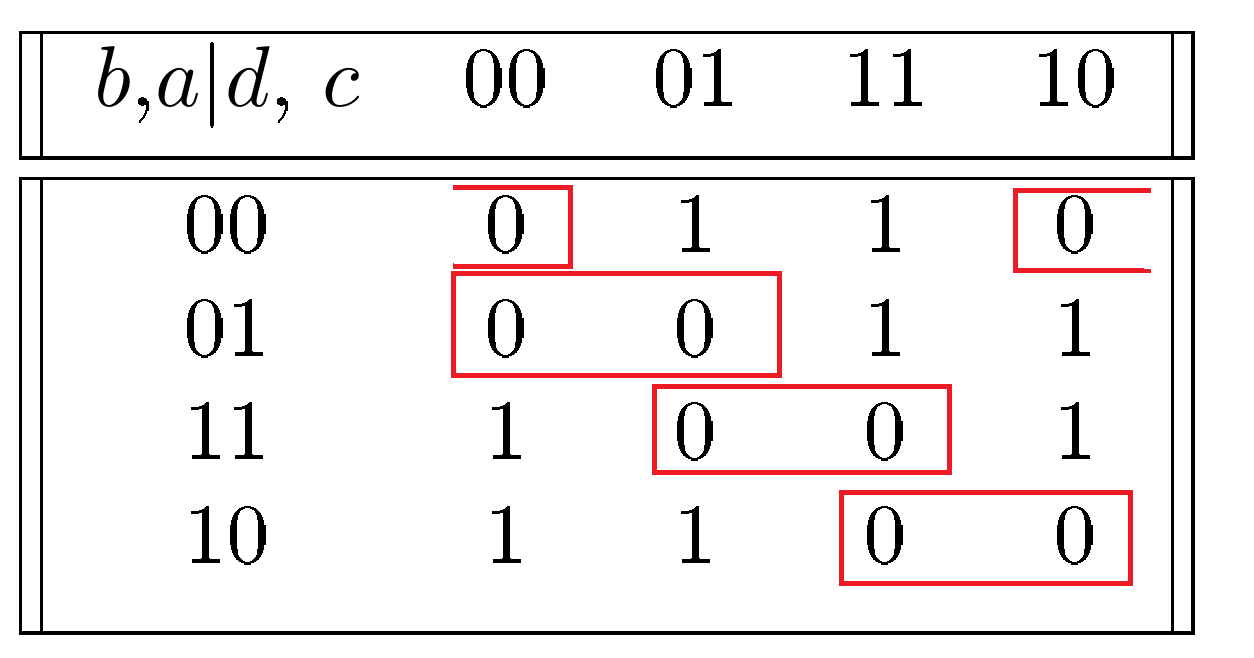
\includegraphics[scale=0.4]{imagenes/karnaugh_ej4.png}
						\caption{Mapa de karnaugh para maxtérminos}
						\label{fig:ej4_karnaugh_ej4}
					\end{figure}
				De este mapa se puede obtener: \par
				$f$ = $(c + b + a) \cdot 
									(d + b + \overline{a}) \cdot 
									(\overline{c} + \overline{b} + \overline{a}) \cdot 
									(\overline{d} + \overline{b} + a) $ \par
			Que resulta ser la expresión equivalente de la obtenida con álgebra de boole (la función f es simétrica).
			\end{itemize}
			%dibujamos el circuito
			\item Obtenemos el circuito resultante a partir de la simplificación: \par
			\begin{figure}[H]	%Circuito
				\centering
				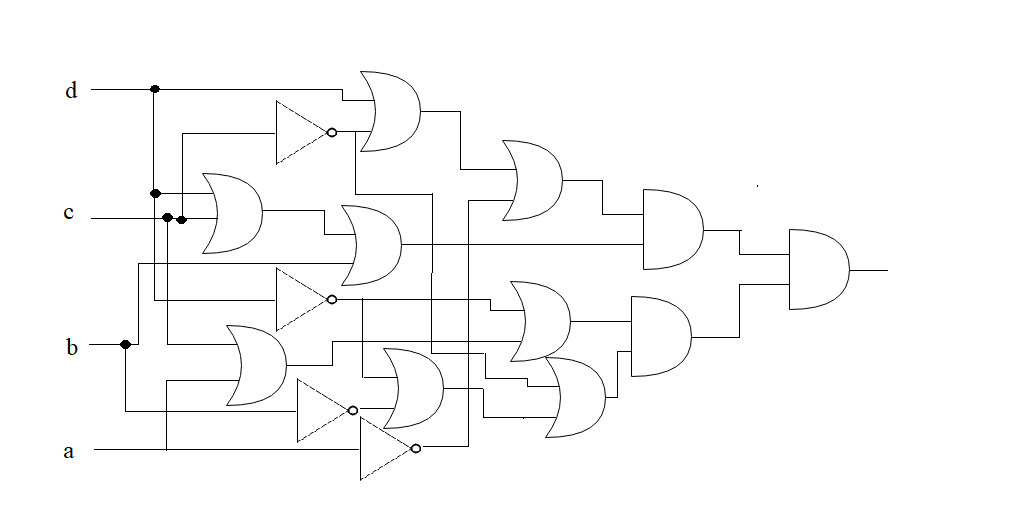
\includegraphics[scale=1]{imagenes/logic_circuit_ej4.png}
				\caption{Circuito lógico resultante}
				\label{fig:ej4_logic_circuit_ej4}
			\end{figure}
			
			%obtenemos el circuito solo con NOR
			\item Obtenemos el mismo circuito a partir de compuertas NOR: \par
					\begin{figure}[H]	%Circuito
						\centering
						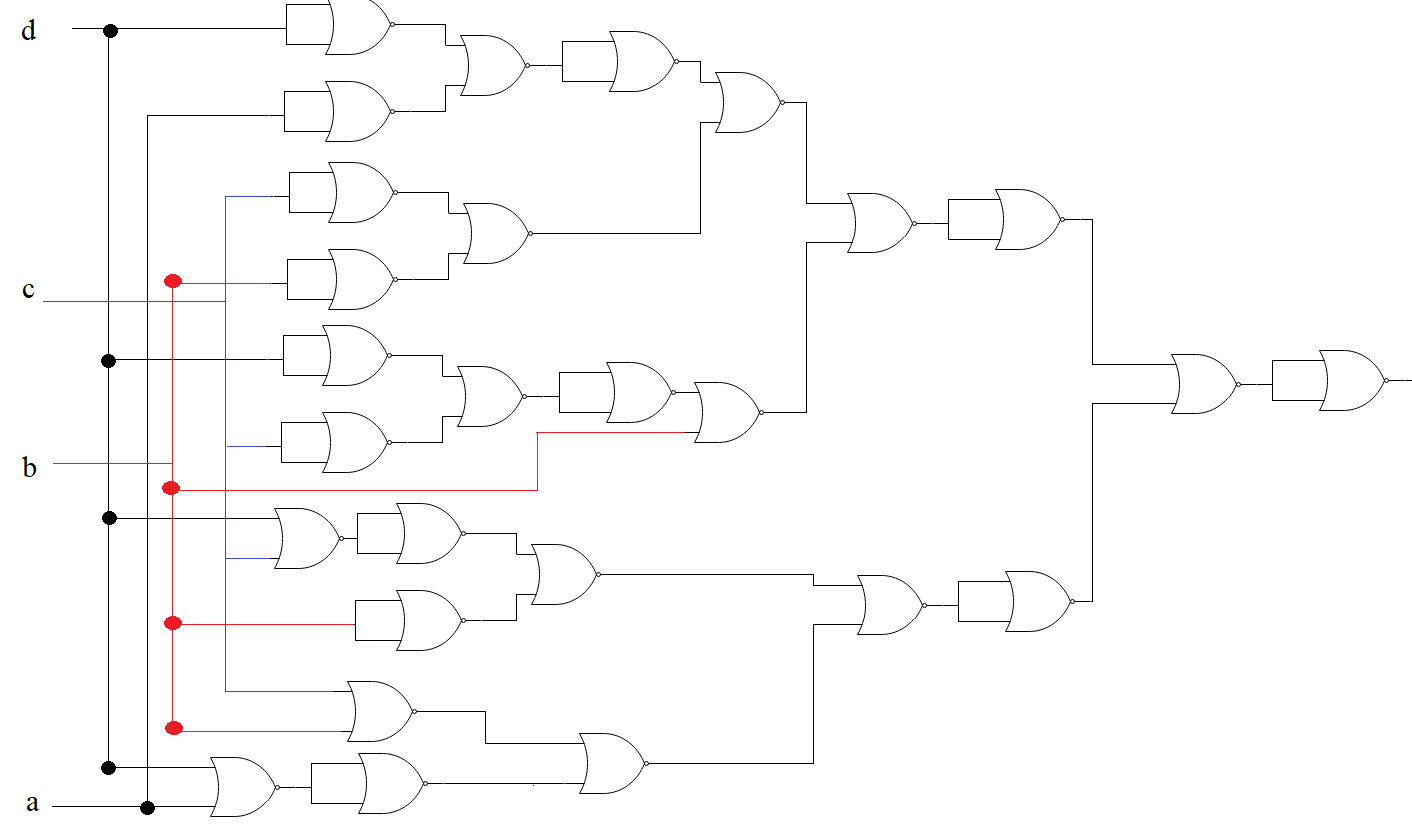
\includegraphics[scale=0.8]{imagenes/circuito_nor_ej4.png}
						\caption{Circuito final implementado con compuertas NOR}
						\label{fig:ej4_circuito_nor_ej4}
					\end{figure}
	 \end{enumerate}
	 
\end{document}


